%==============================================================
\section{Melodic Similarity}\label{melsimc}

As presented in Section~\ref{midiest}, there are tools for the extraction of the pitch curve of the main melody line in a song. However, in polyphonic music these kinds of algorithms struggle to get reasonable results. %even in pop music. 
In musical genres like Metal with distorted instruments it is hardly possible to get good results. 
In conclusion, the main pitch-line extraction and the following conversion of a song with multiple concurrent audio tracks to MIDI using up-to-date open-source toolkits does not produce very reasonable results as shown in~\ref{midiest}.
Another possible representation of melodic features is the transformation of the structural information to graphs, as Orio and Roda did~\cite{graph1}.\\ 
But a better, and also widely used approach is to use chroma features.%as described in the next Section~\ref{chromafeat}.

\subsection{Chroma Features Pre-Processing}\label{chromafeat}

Chroma features, as described in Section~\ref{featsec}, are a good and lower-dimensional way to describe the melody of a song. Most MIR toolkits already offer functions to extract the chromagram from audio files. The plots in this chapter were created using the Essentia~\cite{essentia1} and librosa~\cite{librosa1} toolkits. 
The reduction of dimensionality however, comes with a loss of information, especially which octaves the notes are played in. In addition to the pure computation of the chroma features, some pre- and post-processing steps were implemented and tested and will be presented throughout in this chapter.\\
First of all, Figure~\ref{fig:chroma1} shows the chromagram plots from two different recordings of the first thirty seconds of the song "Chandelier". Figure~\ref{sia} shows the original version sung by the artist Sia and Figure~\ref{pv} shows the features of a cover version by the band Pvris. 
\begin{figure}[htbp]
	\centering
	\framebox{\parbox{1\textwidth}{ 
			\begin{subfigure}{.495\textwidth}
				\centering 
				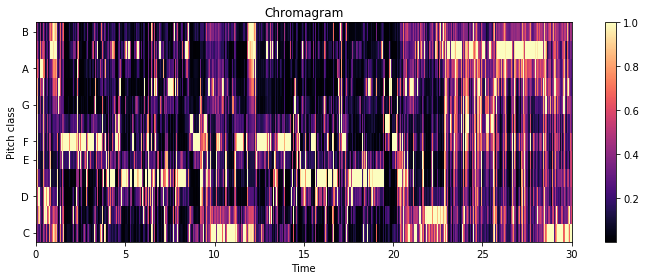
\includegraphics[scale=0.3]{Images/Chroma/sia.png}
				\caption{Chroma features Sia - Chandelier}
				\label{sia}
			\end{subfigure}%
			\begin{subfigure}{.495\textwidth}
				\centering 
				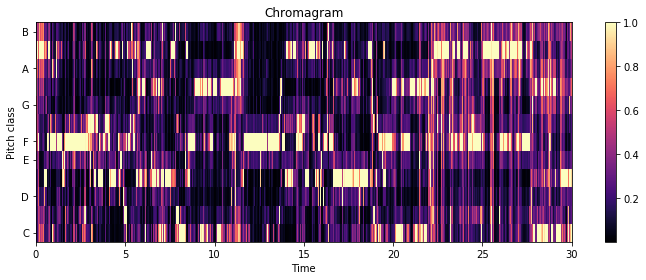
\includegraphics[scale=0.3]{Images/Chroma/pvris.png}
				\caption{Chroma features Pvris - Chandelier}
				\label{pv}
			\end{subfigure}%	
	}}
	\caption{Chroma feature examples}
	\label{fig:chroma1}
\end{figure}
\noindent In the last third of each sample the chroma features seemingly get noisier. At these timings in both songs, the bass and drum begin to play. To reduce the impact of rhythm elements over the melodic voice and instrument lines, the audio signal was filtered with a high-pass filter with a cut-off frequency at 128Hz (nearly equal to C3 Key) and secondly by a low-pass filter with a cut-off frequency at 4096Hz (C8 Key). This limits the frequency range to about 5 octaves. 
In Figure~\ref{fig:sia2}, the filter frequencies and the original audio signals are visualized in blue color, and the filtered audio signal is green. The spectrogram before and after filtering the audio signal is also shown. 
\begin{figure}[htbp]
	\centering
	\framebox{\parbox{1\textwidth}{
			\begin{subfigure}{.495\textwidth}
				\centering
				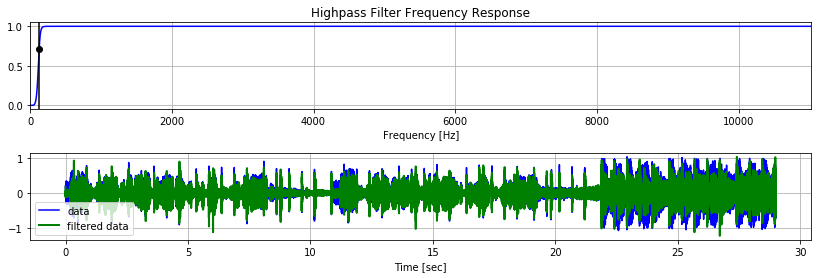
\includegraphics[scale=0.25]{Images/Chroma/siahp.png}
				\caption{High-pass filter}
				\label{siahp}
			\end{subfigure}%
			\begin{subfigure}{.495\textwidth}
				\centering
				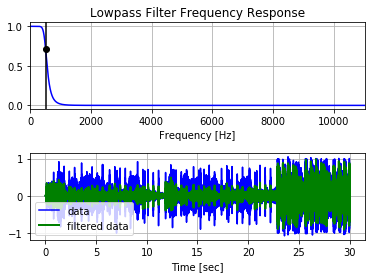
\includegraphics[scale=0.25]{Images/Chroma/sialp.png}
				\caption{Low-pass filter}
				\label{pvhp}
			\end{subfigure}% 
			
			\begin{subfigure}{.495\textwidth}
				\centering
				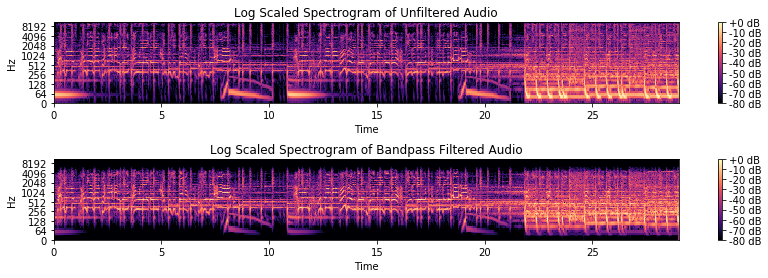
\includegraphics[scale=0.3]{Images/Chroma/siafft.png}
				\caption{FFT band-pass filter Sia}
				\label{siafft}
			\end{subfigure}%
			\begin{subfigure}{.495\textwidth}
				\centering
				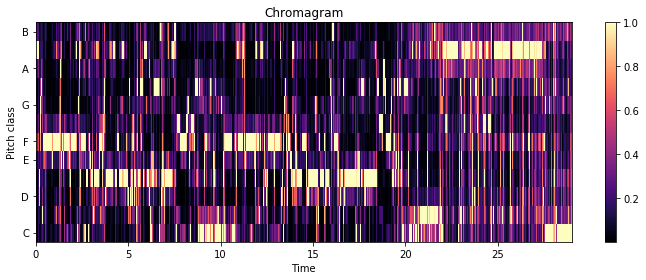
\includegraphics[scale=0.3]{Images/Chroma/chroma_bp.png}
				\caption{Band-pass filtered chromagram}
				\label{pvfft}
			\end{subfigure}%			
	}}
	\caption{Band-pass filtered audio, Sia - Chandelier}
	\label{fig:sia2}
\end{figure}

\noindent In the chromagram of the band-pass filtered audio signal, the last 10 seconds look cleaner and the melody line is more distinct from the rest in comparison to the chromagram of the unfiltered audio in Figure~\ref{fig:chroma1}.\\
The next step is to calculate the most dominant note value for each timeframe. Since the chromagram normalizes every timeframe to the maximum note value, the most dominant note is always assigned to value 1. The closer the rest of the notes are to 1, the more likely the timeframe contains silence. If only a few values are close to 1, a chord or harmony is played. To filter out silence the sum over all note values of every timeframe is calculated and if this sum is twice as high as the average sum of notes of the whole song, the frame is considered as silence. Otherwise, the most dominant pitch is set to a fixed value while the rest of the notes are set to zero.\\
\noindent Usually only the most dominant pitch is needed to extract the main melody, but sometimes the main melody is superimposed by other accompanying instruments. To prevent this, the second most dominant pitches can also be taken into consideration if their values are greater then a specific threshold. The result is shown in Figure~\ref{fig:chromavg} with a threshold of 0.8.
\begin{figure}[htbp]
	\centering
	\framebox{\parbox{1\textwidth}{ 			
			\begin{subfigure}{.495\textwidth}
				\centering    
				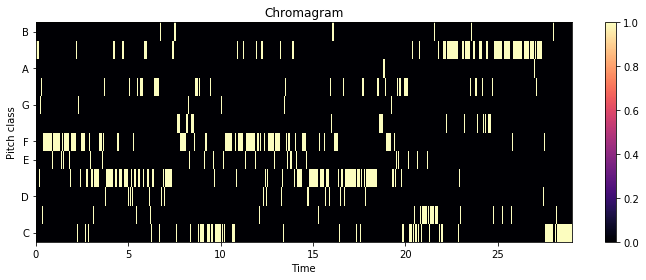
\includegraphics[scale=0.3]{Images/Chroma/sia_1_max.png}
				\caption{Single most dominant note only}
				\label{pvub}
			\end{subfigure}		
			\begin{subfigure}{.495\textwidth}
				\centering     
				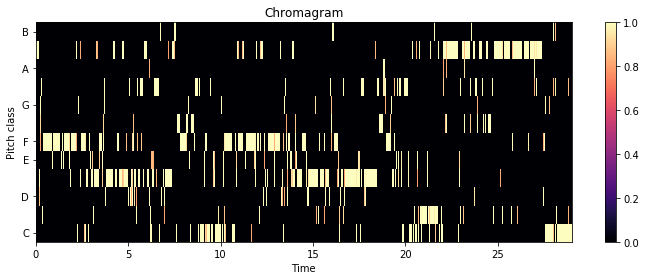
\includegraphics[scale=0.3]{Images/Chroma/sia_2_max.png}
				\caption{First two most dominant notes}
				\label{pvavg}
			\end{subfigure}%			
	}}
	\caption{Thresholded chroma features, Sia - Chandelier}
	\label{fig:chromavg}
\end{figure}
\FloatBarrier

\noindent After that, a beat tracking algorithm is applied to the song and the count of appearances of each note between two beats is calculated. The notes that appear the most between two beats are then set to 1, while the rest is set to 0 for each section between two beats. This beat-alignment serves to make the similarity measurement invariant to the overall tempo of the song. Even if the cover of a song is played with half the tempo of the original song, the melody segment of each bar is still the same as in the faster original version.

\begin{figure}[htbp]
	\centering
	\framebox{\parbox{1\textwidth}{ 			
			\begin{subfigure}{.495\textwidth}
				\centering    
				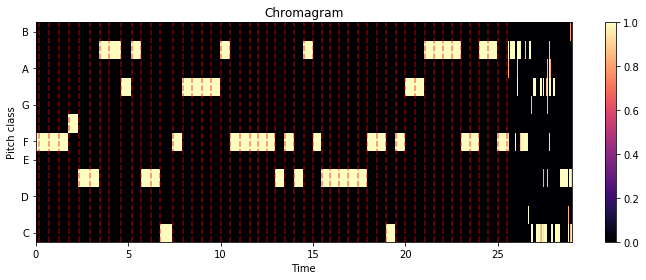
\includegraphics[scale=0.3]{Images/Chroma/pvrisunfiltered.png}
				\caption{Beat-aligned chromagram, unfiltered, Pvris}
				\label{pvubf}
			\end{subfigure}		
			\begin{subfigure}{.495\textwidth}
				\centering     
				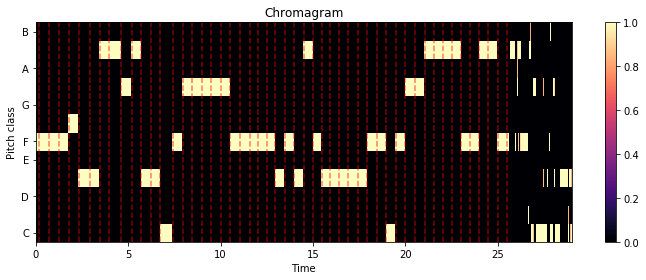
\includegraphics[scale=0.3]{Images/Chroma/pvrisfiltered.png}
				\caption{Beat-aligned chromagram, filtered, Pvris}
				\label{pvfb}
			\end{subfigure}%	
			
			\begin{subfigure}{.495\textwidth}
				\centering    
				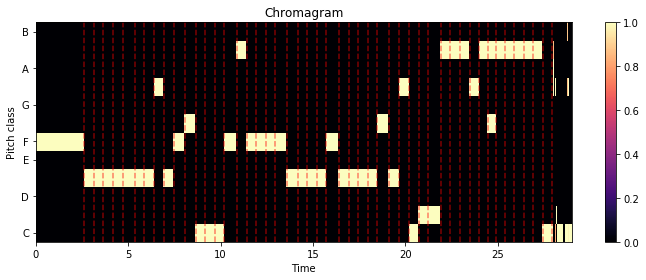
\includegraphics[scale=0.3]{Images/Chroma/siaunfiltered.png}
				\caption{Beat-aligned chromagram, unfiltered, Sia}
				\label{siaub}
			\end{subfigure}
			\begin{subfigure}{.495\textwidth}
				\centering     
				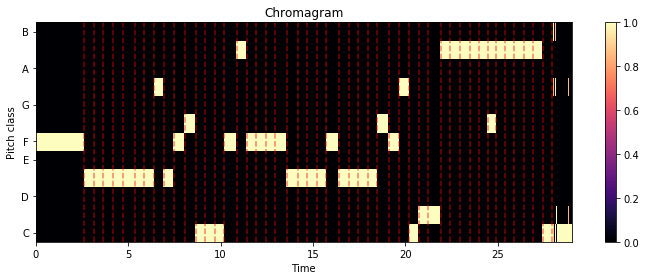
\includegraphics[scale=0.3]{Images/Chroma/siafiltered.png}
				\caption{Beat-aligned chromagram, filtered, Sia}
				\label{siafb}
			\end{subfigure}%		
	}}
	\caption{Processed chroma features, Sia - Chandelier}
	\label{beataligned}
\end{figure}
\FloatBarrier
\noindent Figure~\ref{beataligned} shows the different beat-aligned features of both example songs with band-pass filtered audio and unfiltered audio. The red lines resemble the detected beat events.
\noindent Another option would be to separate the frames between the beats in even smaller sections. This would result in a better resolution of the melodic movement but at the same time increase the length of the data vectors that have to be compared to each other.
\noindent The last processing step is to key shift the chroma features to make the similarity analysis key invariant. One way to do so would be to estimate the key in which each song is played and then shift all chroma features to the same base key, e.g., C Major or A Minor. Due to the structure of the chroma features, this can easily be done by assigning all estimated notes a new value a few keys higher or lower and thus shifting the whole song by a few semitones. The whole workflow to extract the chroma features for this thesis is shown in Figure~\ref{workflowchrom}.\\
\begin{figure}[htbp]
	\centering
	\framebox{\parbox{1\textwidth}{ 	
		\centering
		\ \\
		%\smartdiagramset{set color list={blue!40!white, blue!40!white,blue!40!white, blue!40!white, blue!40!white, blue!40!white}}
		\tikzset{priority arrow/.append style={rotate=180,anchor=0,xshift=30,}}			
		\smartdiagram[priority descriptive diagram]{6) key shifting, 5) beat alignment, 4) extract most dominant pitches, 3) detect silence, 2) calculate chromagram, 1) filter audio (band-pass)} \\
		\caption{Workflow chroma feature extraction}
		\label{workflowchrom}
	}}
\end{figure}
\FloatBarrier
\noindent Another consideration is to use the original chromagram without the extraction of only the most dominant keys and thus leaving the processing step 4 out. This means a possible tradeoff between accuracy and computation time. The results for the example song by Sia do not show a major impact as can be seen in Figure~\ref{fig:nomax}. In this thesis, step 4 will be used in an attempt to get rid of the pitches of the accompaniment from the main melody line.
\begin{figure}[htbp]
	\centering
	\framebox{\parbox{1\textwidth}{ 			
			\begin{subfigure}{.495\textwidth}
				\centering    
				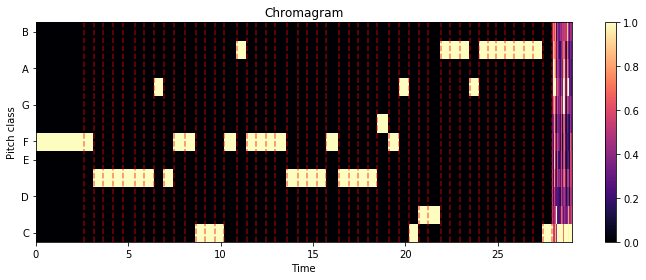
\includegraphics[scale=0.3]{Images/Chroma/nomax.png}
				\caption{Using full chromagram}
				\label{pvubfull}
			\end{subfigure}		
			\begin{subfigure}{.495\textwidth}
				\centering     
				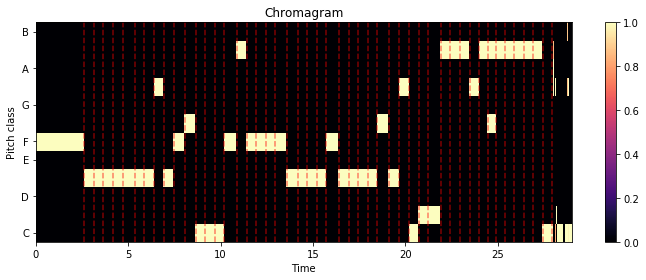
\includegraphics[scale=0.3]{Images/Chroma/siaunfiltered.png}
				\caption{Using most dominant pitches}
				\label{pvdom}
			\end{subfigure}%			
	}}
	\caption{Processing step 3 of chroma features in detail}
	\label{fig:nomax}
\end{figure}

\subsection{Similarity of Melodic Features}

In this section, two completely different approaches to measure the melodic similarity between two songs will be presented. The first one as proposed by~\cite{chroma1} or~\cite{chroma4}, uses text retrieval methods to compare the chroma features of two songs and the second evaluates the usage of cross-correlation of beat-aligned chromagrams as a signal processing approach~\cite{chroma2} and~\cite{chroma3}

\subsubsection{Text Retrieval}\label{textretr}

One possibility to process the chromagrams and to estimate the similarity between the melodic features of different songs is to handle the pre-processed chromagrams as texts consisting of note values. Due to the extraction of only the main melody line in our feature vector, there is only one note for every detected beat. This main melody line gets converted into a vector of subsequent notes and the resulting vector is converted into a string. The beat- and pitch-alignment done in the previous steps makes the features relatively time- and key invariant. One problem that remains is the different length of the various feature vectors. Xia (et al)~\cite{chroma4} mentions that this is indeed a problem when using the Levenshtein distance (also known as the edit-distance) to compute similarities. The Levenshtein distance between the first $i$ characters of a string $S$ and the first $j$ characters of $T$ can be calculated as:

\begin{equation} \label{eq:tr1}
\text{lev}_{S,T}(i, j) = \begin{cases}
\quad\text{max}(i, j), & \text{if} \, \text{min}(i, j) = 0\\
\quad\text{min}(\\
	\quad\quad\text{lev}_{S,T}(i-1, j) + 1,\\ 
	\quad\quad\text{lev}_{S,T}(i, j-1) + 1,	& \text{else},\\
	\quad\quad\text{lev}_{S,T}(i-1, j-1) + 1_{(S_i \neq T_j)}\\
	\quad)\\ 
	\end{cases}
\end{equation}

\noindent with $1_{(S_i \neq T_j)}$ being the indicator function equal to 0 when $S_{i} = T_{j}$ and equal to 1 otherwise, following~\cite[p. 7]{chroma4}.

%\begin{equation} \label{eq:tr1}
%lev_{S,T}(i, j) = \begin{cases}
%max(i, j), &\text{if } min(i, j) = 0\\
%min \begin{cases}
%lev_{S,T}(i-1, j) + 1\\
%lev_{S,T}(i, j-1) + 1\\
%lev_{S,T}(i-1, j-1)\\
%+cost[S_i \neq T_j]\\
%\end{cases} &\text{else} \\
%\end{cases}
%\end{equation}
\noindent In their paper, Xia (et al.) use MIDI files instead of chroma features, but both contain information about the melody of songs. An adaption to chroma features is not an issue, because they can also easily be interpreted as simple strings. 
\noindent They also made some adjustments to Equation~\ref{eq:tr1} to be able to handle musical information.~\cite[pp. 7ff]{chroma4} For example to get rid of the problem of various lengths between the songs, they only took the first 200 and the last 200 notes of every song because it could be observed that cover songs tend to share more common notes in the beginning and at the end of each song.\\
Due to the fact that this thesis has no actual note information from MIDI files but rather short lists of estimated main pitches from the beat-aligned chroma features, most of the feature vectors are already smaller than 200 notes. Therefore the implemented algorithm does not split the vectors. This tends to favor cover songs that share the same length. 
\ \\
Englmeier (et al.) uses a more advanced text information retrieval technique called "TF-IDF weights" (term frequency - inverse document frequency) and explicit semantic analysis (ESA). "The TF-IDF weight is a measure which expresses the meaning of a term or a document within a collection of documents."~\cite[p. 186]{chroma1}
To do so, "audio words" have to be created from the song database by splitting the audio signal into snippets, creating chroma features and clustering them with the k-means algorithm. The centroids are then added to a database. These audio words can then be evaluated using the TF-IDF weights and ESA.
Although their approach looks promising, a re-implementation of their algorithms would exceed the frame of this thesis.

\subsubsection{Cross-Correlation}\label{crosscorrsec}

Another possibility to handle the extracted chroma features is to view them as ordinary discrete time signals and creating opportunities to apply classical signal processing algorithms. For this approach, the pre-processing steps laid out in Figure~\ref{workflowchrom} can be simplified by skipping steps 3 and 4 and possibly even step 6, as explained later, resulting in beat-aligned chromagrams as shown in Figure~\ref{cch1} and~\ref{cch2}.\\
Ellis and Poliner use the cross-correlation in their 2007 published paper~\cite{chroma3}. Serra (et al.) also references the work of Ellis and Poliner and discusses different weak points and influences of processing steps like beat tracking and key transposition to the overall performance of this similarity measurement. 
They also discuss and improve another approach called "dynamic time warping" (DTW) further in their paper~\cite{chroma2}. The focus of this thesis is set on the cross-correlation method. 
Given two discrete-time signals $x[n]$ and $y[n]$ the cross-correlation between both signals $k[n] = (x \star y)[n]$ can be denoted as follows:
\begin{equation} \label{eq:conv1}
k[n] = (x \star y)[n] = \sum_{m = -\infty}^{\infty}{x[m] y[m - n]}.
\end{equation}
For two two-dimensional input matrices $X$ with the dimensions $M$ by $N$ and $Y$ as a $P$ by $Q$ matrix the cross-correlation result is a matrix $C$ of size $M + P - 1$ rows and $N + Q - 1$ columns. Its elements are given by the equations~\cite{mathcorr}:
\begin{equation} \label{eq:conv2}
C(k, l) = \sum_{m = 0}^{M - 1}{\sum_{n = 0}^{N - 1}{X(m, n)\overline{Y}(m - k, n - l)}}
\end{equation}
with 
\begin{equation} \label{eq:conv3}
-(P - 1) \leq k \leq M - 1
\end{equation}
\begin{equation} \label{eq:conv4}
-(Q - 1) \leq l \leq N - 1.
\end{equation}
The bar over $\overline{Y}$ denotes complex conjugation (in this case $Y$ is a matrix with real values only). 
An example for the one-dimensional cross-correlation is shown in Figure~\ref{fig:corr1} and the full two-dimensional cross-correlation of two songs is depicted in Figure~\ref{fig:beatalign} and~\ref{fig:crosscorr}.
\begin{figure}[htbp]
	\centering
	\framebox{\parbox{1\textwidth}{ \centering			
	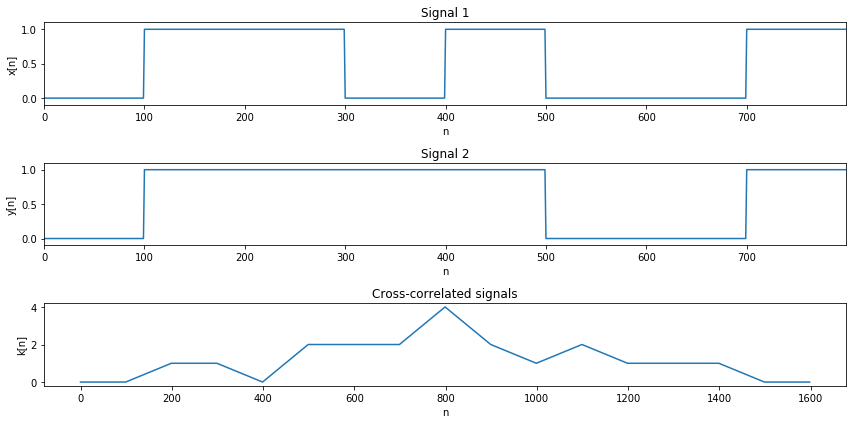
\includegraphics[scale=0.45]{Images/Chroma/correlation.png}
	}}
	\caption{1D cross-correlation}
	\label{fig:corr1}
\end{figure}
Ellis and Poliner did not transpose the songs in the pre-processing step to match the keys of both audio files. Instead, they calculated the full cross-correlation for all 12 possible transpositions and chose the best one. 
As input matrices, they averaged all notes of the chroma features per beat and additionally scaled them to have unit norm at each time slice (beat frame).
In the original paper, the cross-correlation is normalized by the length of the shorter song segment to bind the correlation result to an interval between 0 and 1. But in a later published work from Ellis and Cotton, this step was left out as it seemingly resulted in slightly worse detection ratios of cover songs~\cite{cover802}. 
Additionally, they filtered the result of the cross-correlation with a high-pass filter. "We found that genuine matches were indicated not only by cross-correlations of large magnitudes, but that these large values occurred in narrow local maxima in the cross-correlations that fell off rapidly as the relative alignment changed from its best value. To emphasize these sharp local maxima, we choose the transposition that gives the largest peak correlation then high-pass filter that cross-correlation function with a 3dB point at 0.1 rad/sample"~\cite[p. 3]{chroma3}. The later published paper also states that changes to the filter parameters improved the cover song recognition rate further~\cite{cover802}. However, the exact values, e.g., for the cutoff frequency were not given. Accordingly, in this thesis, the older parameters for the filter are used.\\
Serra (et al.) also discusses the effects of different pre-processing steps that improve the algorithm even further and they note that a higher chroma resolution of 3 octaves gives better results. Also, the key detection and transposition before the cross-correlation gives slightly worse results in comparison to the method Ellis and Poliner used.\\ 
In this thesis, a version where the songs are all key aligned before the cross-correlation was tested to reduce the computation time overhead when estimating the similarities on a cluster. 
%but due to the fact, that the key detection algorithm in the librosa and Essentia frameworks weren't always correct a second version where additionally the cross-correlation for all key transpositions is calculated, was also implemented. 
In summary, the implementation in this thesis is similar to the approach by Ellis and Poliner~\cite{chroma3}, but some of the steps from the newer paper~\cite{cover802} leave some space for further improvements.\\ The chroma features are beat aligned, averaged per beat, and normalized to unit length as well. Additionally, all chroma features are transposed to a common key (A in this case) in the pre-processing step. The full cross-correlation according to Equation~\eqref{eq:conv2} including "key shifts" with zero padding at the edges by letting $k$ run from $-(P - 1) \leq k \leq M - 1$ is shown in Figures~\ref{fig:beatalign} and~\ref{fig:crosscorr}. But due to the previously already performed key shift during the pre-processing steps and the fact that both input matrices share the same amount of rows (12, one per semi-tone), the full cross-correlation is not necessary and computation time can be saved by altering the computation according to Equation~\eqref{eq:conv5} resulting in a vector $C$ with the correlation results without additional key-shifting
\begin{equation} \label{eq:conv5}
C(l) = \sum_{m = 0}^{M - 1}{\sum_{n = 0}^{N - 1}{X(m, n)\overline{H}(m, n - l)}}
\end{equation}
\begin{equation} \label{eq:conv6}
-(Q - 1) \leq l \leq N - 1
\end{equation}
or even faster without calculating the edges of the matrix (without zero-padding).
\begin{equation} \label{eq:conv7}
0 \leq l \leq N - Q
\end{equation}
\noindent This simplified version relies on an accurate key detection of the songs during the pre-processing. The post-processing step from Ellis and Poliner, more precisely the high-pass filtering of the result was also implemented.\\
Figure~\ref{fig:beatalign} shows two beat aligned, key-shifted and per beat averaged chroma features of two short guitar audio samples and their cross-correlation results. The most interesting row of the cross-correlation matrix is the middle row marked with the B key on the y-axis, where both chromagrams are aligned. %It shows that both already key shifted melodies do not correlate well in this example.  
\begin{figure}[htbp]
	\centering
	\framebox{\parbox{1\textwidth}{ 			
			\begin{subfigure}{.495\textwidth}
				\centering    
				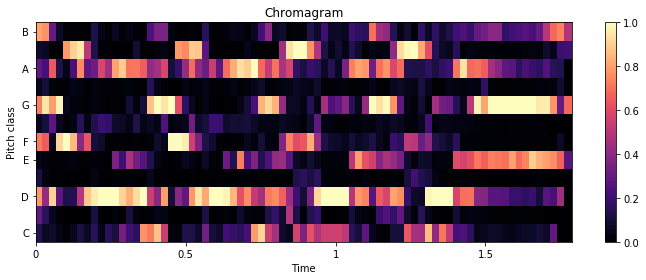
\includegraphics[scale=0.3]{Images/Chroma/beatalignedchroma.png}
				\caption{Beat-aligned chromagram sound1}
				\label{c1}
			\end{subfigure}				
			\begin{subfigure}{.495\textwidth}
				\centering    
				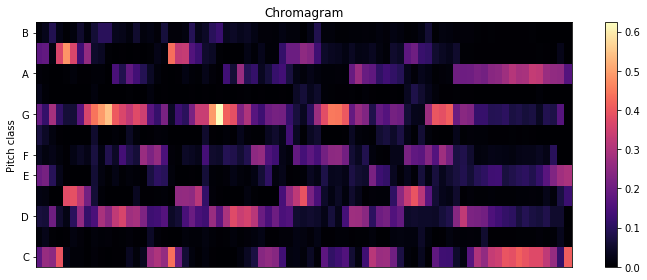
\includegraphics[scale=0.3]{Images/Chroma/beatalignedchroma_ks.png}
				\caption{Beat-aligned chromagram sound1 key-shifted}
				\label{cks1}
			\end{subfigure}		
			
			\begin{subfigure}{.495\textwidth}
				\centering     
				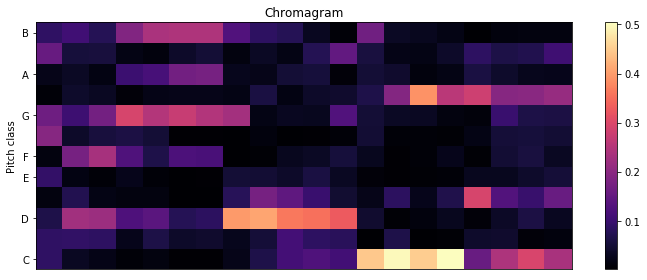
\includegraphics[scale=0.3]{Images/Chroma/beatalignedchroma2_ks.png}
				\caption{Beat-aligned chromagram sound2 key-shifted}
				\label{cks2}
			\end{subfigure}%	
			\begin{subfigure}{.495\textwidth}
				\centering     
				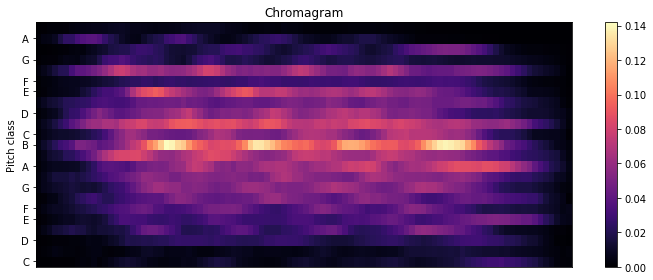
\includegraphics[scale=0.3]{Images/Chroma/beatalignedchroma_corr.png}
				\caption{Cross-correlation}
				\label{c2}
			\end{subfigure}%			
	}}
	\caption{2D cross-correlation of beat-aligned and key-shifted chromagrams (audio snippets)}
	\label{fig:beatalign}
\end{figure}

\noindent In Figure~\ref{fig:crosscorr} the cross-correlation of the song "Chandelier" by singer Sia and covered by Pvris are shown in~\ref{cc1} and in contrast to this the cross-correlation of "Chandelier" with the song "Rock you like a Hurricane" by The Scorpions is shown (Figure~\ref{cc2}). 
\begin{figure}[htbp]
	\centering
	\framebox{\parbox{1\textwidth}{ 			
			\begin{subfigure}{.495\textwidth}
				\centering    
				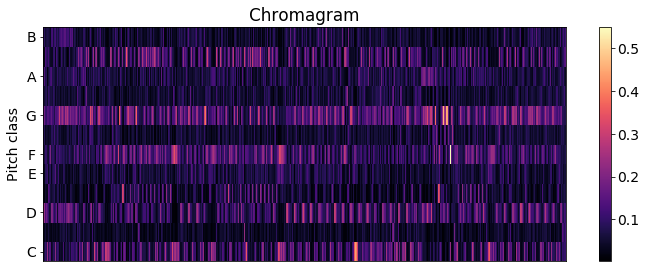
\includegraphics[scale=0.3]{Images/Chroma/hurr1chrom.png}
				\caption{Chandelier, Pvris}
				\label{cch1}
			\end{subfigure}		
			\begin{subfigure}{.495\textwidth}
				\centering     
				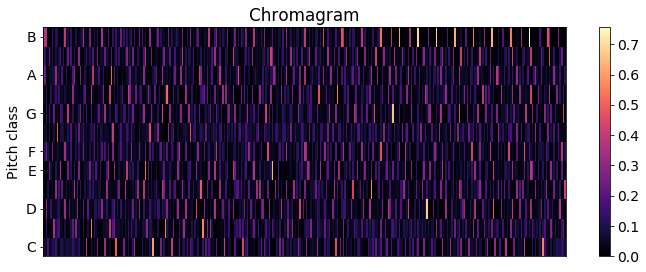
\includegraphics[scale=0.3]{Images/Chroma/hurr2chrom.png}
				\caption{Chandelier, Sia}
				\label{cch2}
			\end{subfigure}%
				
			\begin{subfigure}{.495\textwidth}
				\centering    
				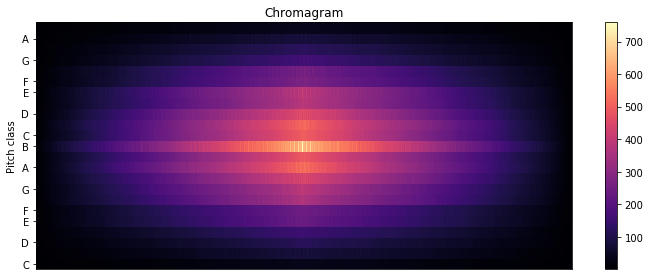
\includegraphics[scale=0.3]{Images/Chroma/cross_hurricane.png}
				\caption{Cross-correlation of cover songs}
				\label{cc1}
			\end{subfigure}		
			\begin{subfigure}{.495\textwidth}
				\centering     
				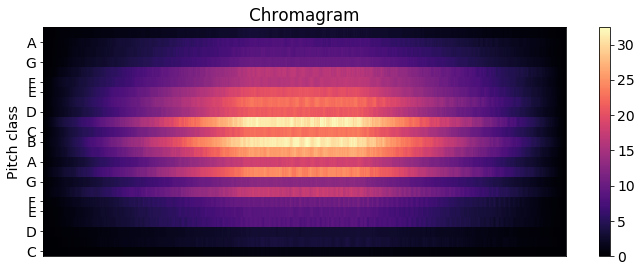
\includegraphics[scale=0.3]{Images/Chroma/cross_hurricane_sia.png}
				\caption{Cross-correlation of unrelated songs}
				\label{cc2}
			\end{subfigure}%			
	}}
	\caption{2D cross-correlation of beat-aligned chromagrams (Sia / Pvris - Chandelier)}
	\label{fig:crosscorr}
\end{figure}
%\FloatBarrier

\noindent Due to the previous key shifting, plot~\ref{cc1} shows the maximum peak right in the center row. Originally, the version by Sia is detected to be written in C sharp and the cover version in F sharp, but both songs are shifted to the A key during the pre-processing step.\\
\noindent The unrelated songs result in much smaller correlation values, especially when looking at the middle row of the matrix (marked with the F key on the y-axis in figure \ref{cc2}), but also if the songs were transposed additionally even then they would not correlate well, but this is also related to the zero-padding when additional key-shifts are performed. 
In contrast to this, the cover songs have multiple visible peaks in the center row. 
\noindent The row with the maximum correlation value is extracted, and the resulting plot shows that the cover songs do correlate much better than the unrelated songs (\ref{cc3} and~\ref{cc4}).
The center rows of the cross-correlation matrices from Figure~\ref{fig:crosscorr} are separately pictured in Figure~\ref{fig:crosscorr3}. After applying the high-pass filter to the extracted row with the maximum correlation value, the peaks in~\ref{cc3} when cross-correlating the cover songs are clearly visible compared to the unrelated songs. An interesting detail that can be pointed out is that the song structure is also visible in plot~\ref{ccf3} with clearly visible recurring peaks when the refrain is repeated.
\begin{figure}[htbp]
	\centering
	\framebox{\parbox{1\textwidth}{ 			
			\begin{subfigure}{.495\textwidth}
				\centering    
				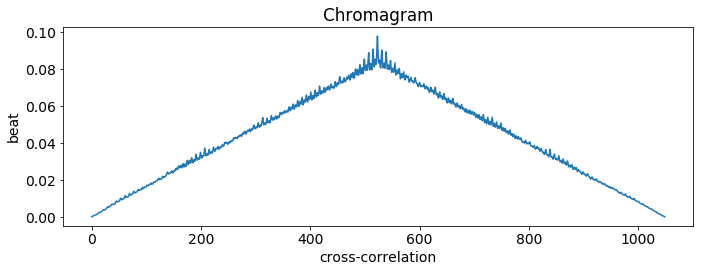
\includegraphics[scale=0.3]{Images/Chroma/beatalignedchroma_corr_mean.png}
				\caption{Cross-correlation of cover songs}
				\label{cc3}
			\end{subfigure}		
			\begin{subfigure}{.495\textwidth}
				\centering     
				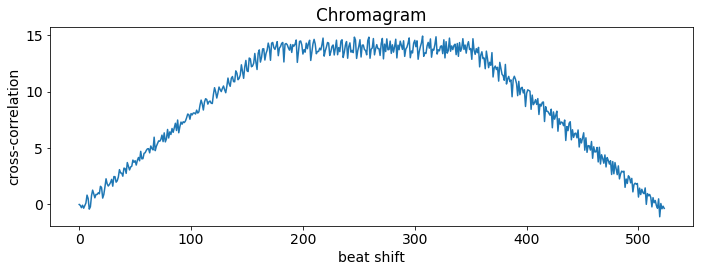
\includegraphics[scale=0.3]{Images/Chroma/beatalignedchroma_corr_mean2.png}
				\caption{Cross-correlation of unrelated songs}
				\label{cc4}
			\end{subfigure}%			
%	}}
%	\caption{Cross-correlation}
%	\label{fig:crosscorr2}
%\end{figure}
%\FloatBarrier

%\begin{figure}[htbp]
%	\centering
%	\framebox{\parbox{1\textwidth}{ 				
			\begin{subfigure}{.495\textwidth}
				\centering    
				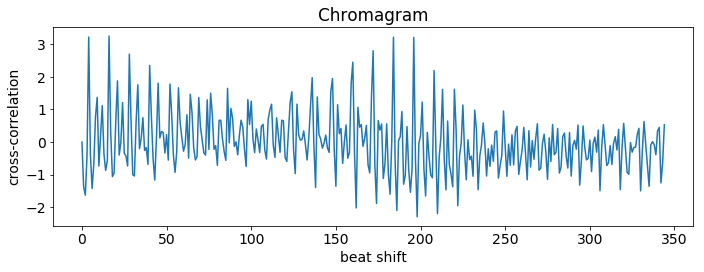
\includegraphics[scale=0.3]{Images/Chroma/beatalignedchroma_corr_mean_filt.png}
				\caption{Cover songs filtered}
				\label{ccf3}
			\end{subfigure}		
			\begin{subfigure}{.495\textwidth}
				\centering     
				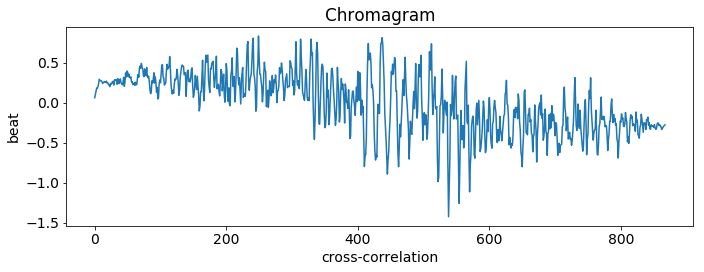
\includegraphics[scale=0.3]{Images/Chroma/beatalignedchroma_corr_mean2_filt.png}
				\caption{Unrelated songs filtered}
				\label{ccf4}
			\end{subfigure}%		
	}}
	\caption{Filtered cross-correlation (high-pass)}
	\label{fig:crosscorr3}
\end{figure}
%\FloatBarrier

\subsection{Validation}\label{chromavalid}
A good measurement for the efficiency of a melodic similarity algorithm is the ability to find cover songs, remixes, and different recordings of the same song. Chapter~\ref{covsongid} evaluates the cover song recognition rate of the implemented recommender system. 
